\subsection{Cost of connection setup}
In applications designed to allow people to communicate, the time a message takes to be delivered is a fundamental parameter.
The delivery time can be split in two parts: the setup of the Bluetooth connection and the transfer time for the message.
Analyzing the impact of the time required for the setup of the connection over the total time required for the delivery of the message is particularly important in the context of multi-hop communication systems, where each node has to hold (hence setup) a large amount of connections with other peers of the system.

The benchmark tested the connection setup cost and the time required to transfer messages of different sizes between two devices.
In order to make sure that the network wasn't loaded and the connection setup cost was being evaluated correctly only one device at a time could send messages.
At the beginning of the test, a token is created by the master. At most one device can hold the token at a certain time. This ensures that only one device at a time is allowed to send messages.
During a run of the test, the devices are organized in a circular ring, and every time a device receives the token it sends a message to the next device in the ring and takes some measures about connection time and transfer time. Then, it sends the token to the next device that will repeat the process.
The pseudo code for a peer in the ring is shown in Algorithm \ref{pseudo:ring_peer}.

\begin{algorithm}
	\begin{algorithmic}[1]
  		\caption{Ring peer pseudocode}
  		\label{pseudo:ring_peer}
  		\While {true}
		\State $socket \leftarrow serverSocket.accept()$
		\State $ping \leftarrow socket.read(payloadSize)$
		\State $socket.write(pong)$
		\State $token \leftarrow receiveToken()$
		\State $nextDevice \leftarrow nextPeer()$ \Comment next peer in ring
		\State $T_0 \leftarrow nanotime()$ \Comment current time in nanoseconds
		\State $newSocket \leftarrow nextDevice.connect()$
		\State $T_1 \leftarrow nanotime()$ 
		\State $newSocket.write(ping(randomByteArray(payloadSize)))$
		\State $pong \leftarrow socket.read()$
		\State $T_2 \leftarrow nanotime()$
		\State $token.times.add(T_0, T_1, T_2)$
		\State $socket.write(token)$
		\EndWhile
  	\end{algorithmic}
\end{algorithm}

The master is designated when the test starts and it is responsible for sending the first ping to the following device in the ring, in order to start the test.
It is responsibility of the master to stop the loop as well, when the token has traveled through the ring for a defined number of times.

\subsubsection{Test execution}
In order to be sure to collect a sufficient amount of data, the test was performed multiple times and with different configurations.
The test has been performed on 4 sets of devices, forming 4 different ring configurations.
For each of those ring configurations, the test has been executed a total of 40 times, 10 times for each payload size.
Before every test, all the devices have been rebooted.
A test was considered finished when the token passed through every peer of the ring 5 times.

In a portion of the tests that have been executed, a problem has arisen, preventing the test from finishing successfully.
In those cases, the token would be blocked inside the ring mainly due to errors in the setup of the connection, preventing the test from continuing.
When this occurred, data collected up to that point was saved and the the test continued with the next run.
It is important to note that if a test consisting in $N$ token hops failed at the $n$th one, the remaining $N - n$ hops weren't completed and were accounted as failed transmissions.
However, the problem would be less of an issue in network topologies other than a ring, where the failure of a node won't necessarily compromise the entire network.

The correlation between rate of messages lost and configuration of the ring of devices is shown in Table \ref{table:failure_rate_ring_config}.
The correlation between failures and size of payload transmitted, on the other hand, is shown in Table \ref{table:failure_rate_payload_size}.

\begin{table}[h]
\centering
\begin{tabular}{llll}
\hline
Devices                             & Master      & Total   &  Failed    \\ \hline
Nexus 5, Nexus 4, Nexus 7           & Nexus 5     & 600     & 342        \\
Nexus 4, Nexus 5, Nexus 7           & Nexus 4     & 600     & 114        \\
Nexus 4, Nexus 5, Nexus 7, Redmi    & Nexus 4     & 800     & 256        \\
Redmi, Nexus 5, Nexus 7, Nexus 4    & Redmi       & 800     & 296        \\
\hline
\end{tabular}
\caption{Rate of messages that went lost by configuration of ring of devices}
\label{table:failure_rate_ring_config}
\end{table}


\begin{table}[h]
\centering
\begin{tabular}{llll}
\hline
Size of payload (bytes) & Total     & Failed    \\ \hline
512                     & 700       & 213       \\
1024                    & 700       & 310       \\
2048                    & 700       & 251       \\
4096                    & 700       & 234       \\
\hline
\end{tabular}
\caption{Rate of messages that were lost by size of the payload transmitted}
\label{table:failure_rate_payload_size}
\end{table}

\subsubsection{Results}
This test highlighted the impact that the time taken to setup a connection has on the total time needed to send a message between two devices.
The cost of connection setup becomes less significant when the same connection is preserved and used for a longer period of time (i.e. when the communication is performed between two devices only), since the connection setup will affect only the first communication.

\begin{figure}[ht!]
  \centering
  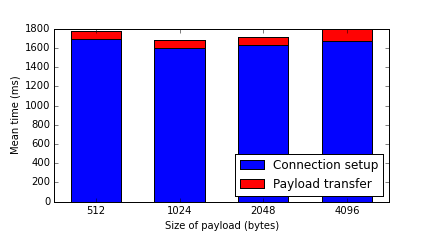
\includegraphics[width=1.0\textwidth]{application/img/setup_with_transfer.png}
  \caption{Average time for connection setup and message transmission for different sizes of payload}
  \label{figure:conn_vs_transfer}
\end{figure}

Fig. \ref{figure:conn_vs_transfer} shows the impact that the time taken to setup a connection has over the total time needed to send a message of different sizes.
For each set of measurements $(T_0, T_1, T_2, N)$, which represent respectively the time before the connection, after the connection and after the transmission of the message and the number of bytes transferred, the cost in time of connection setup was computed, for every payload size, as the mean of all the values $T_C = T_1 - T_0$.
The cost of transmission of the message was computed, for every payload size, as the mean of the values $T_T = T_2 - T_1$.

\begin{figure}[ht!]
  \centering
  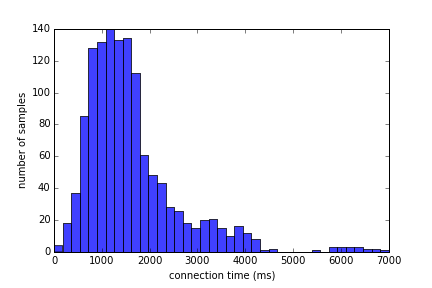
\includegraphics[width=1.0\textwidth]{application/img/setup_distribution.png}
  \caption{Distribution of time required to setup a connection between two devices. Three outliers are not shown in this figure due to their high value. More specifically, their values are 19105, 18956 and 7172 ms}
  \label{figure:conn_time_distribution}
\end{figure}

Fig \ref{figure:conn_time_distribution} shows the distribution of connection time observed during all the tests performed.
Size of payload was not considered because the time to setup the connection was measured before the transmission of any data. Three outliers are not shown in the figure for representation purposes. Their values are 19105, 18956 and 7172 ms.
As can be seen, the vast majority of connections required a time between 1 and 2 seconds to setup.
However, a non negligible amount of connections required a considerable amount of time to setup.
Even though this behaviour was observed in a relatively small amount of samples, it should be taken into consideration when designing a system relying on the Bluetooth technology, particularly if this system is required to setup new connections frequently.